\subsubsection{Трехуровневая архитектура}

Если говорить про многоуровневую архитектуру взаимодействия клиент-сервер, то в качестве примера можно привести любую современную СУБД (за исключением библиотеки SQLite, которая в принципе не использует концепцию клиент-сервер). Суть многоуровневой архитектуры заключается в том, что запрос клиента обрабатывается сразу несколькими серверами. Такой подход позволяет значительно снизить нагрузку на сервер из-за того, что происходит распределение операций, но в то же самое время данный подход не такой надежный, как двухуровневая архитектура (рисунок 6.1). Трехзвенная архитектура сложнее, но это достойная цена за пользу, которую может принести распределение функций между серверами второго и третьего уровня.

Трехзвенная архитектура клиент-сервер имеет следующие основные преимущества:
\begin{enumerate}
	\item Высокая степень гибкости и масштабируемости. Может быть расширена путем выделения дополнительных серверов, каждый из которых будет представлять собственные сервисы и пользоваться услугами прочих серверов разного уровня.
	\item Высокая степень безопасности. Защиту можно определить для каждого сервиса или уровня.
	\item Высокая производительность. Задачи распределены между серверами.
\end{enumerate}

Взаимодействие клиента с сервером, при такой архитектуре, происходит путем запросов. Т.е. клиент отправляет запрос на сервер, для совершения некоторого действия, сервер получает запрос, взаимодействует с базой данных, обрабатывает полученные данные из базы и после отправляет обратно к клиенту.

Типичный пример трехуровневой модели клиент-сервер. Если говорить в контексте систем управления базами данных, то первый уровень – это клиент, который позволяет нам писать различные SQL запросы к базе данных. Второй уровень – это движок СУБД, который интерпретирует запросы и реализует взаимодействие между клиентом и файловой системой, а третьим уровнем является хранилище данных.

Учтя всё вышесказанное, можно смоделировать клиент-серверную структуру для нашего приложения. Она будет представлена трехуровневой системой. На первом уровне располагаются веб-клиент СЭД и клиент MRScan. Веб клиент занимается основной обработкой всего функционала документооборота, направляя запросы на сервер(3-й уровень), сервер в свою очередь обращается к серверу базы данных для получения необходимых данных. Клиент MRScan передает серверу отсканированные файлы по технологии WCF. Схема архитектуры проекта представлена на рисунке 6.2.

\begin{figure}[h!]
	\centering
	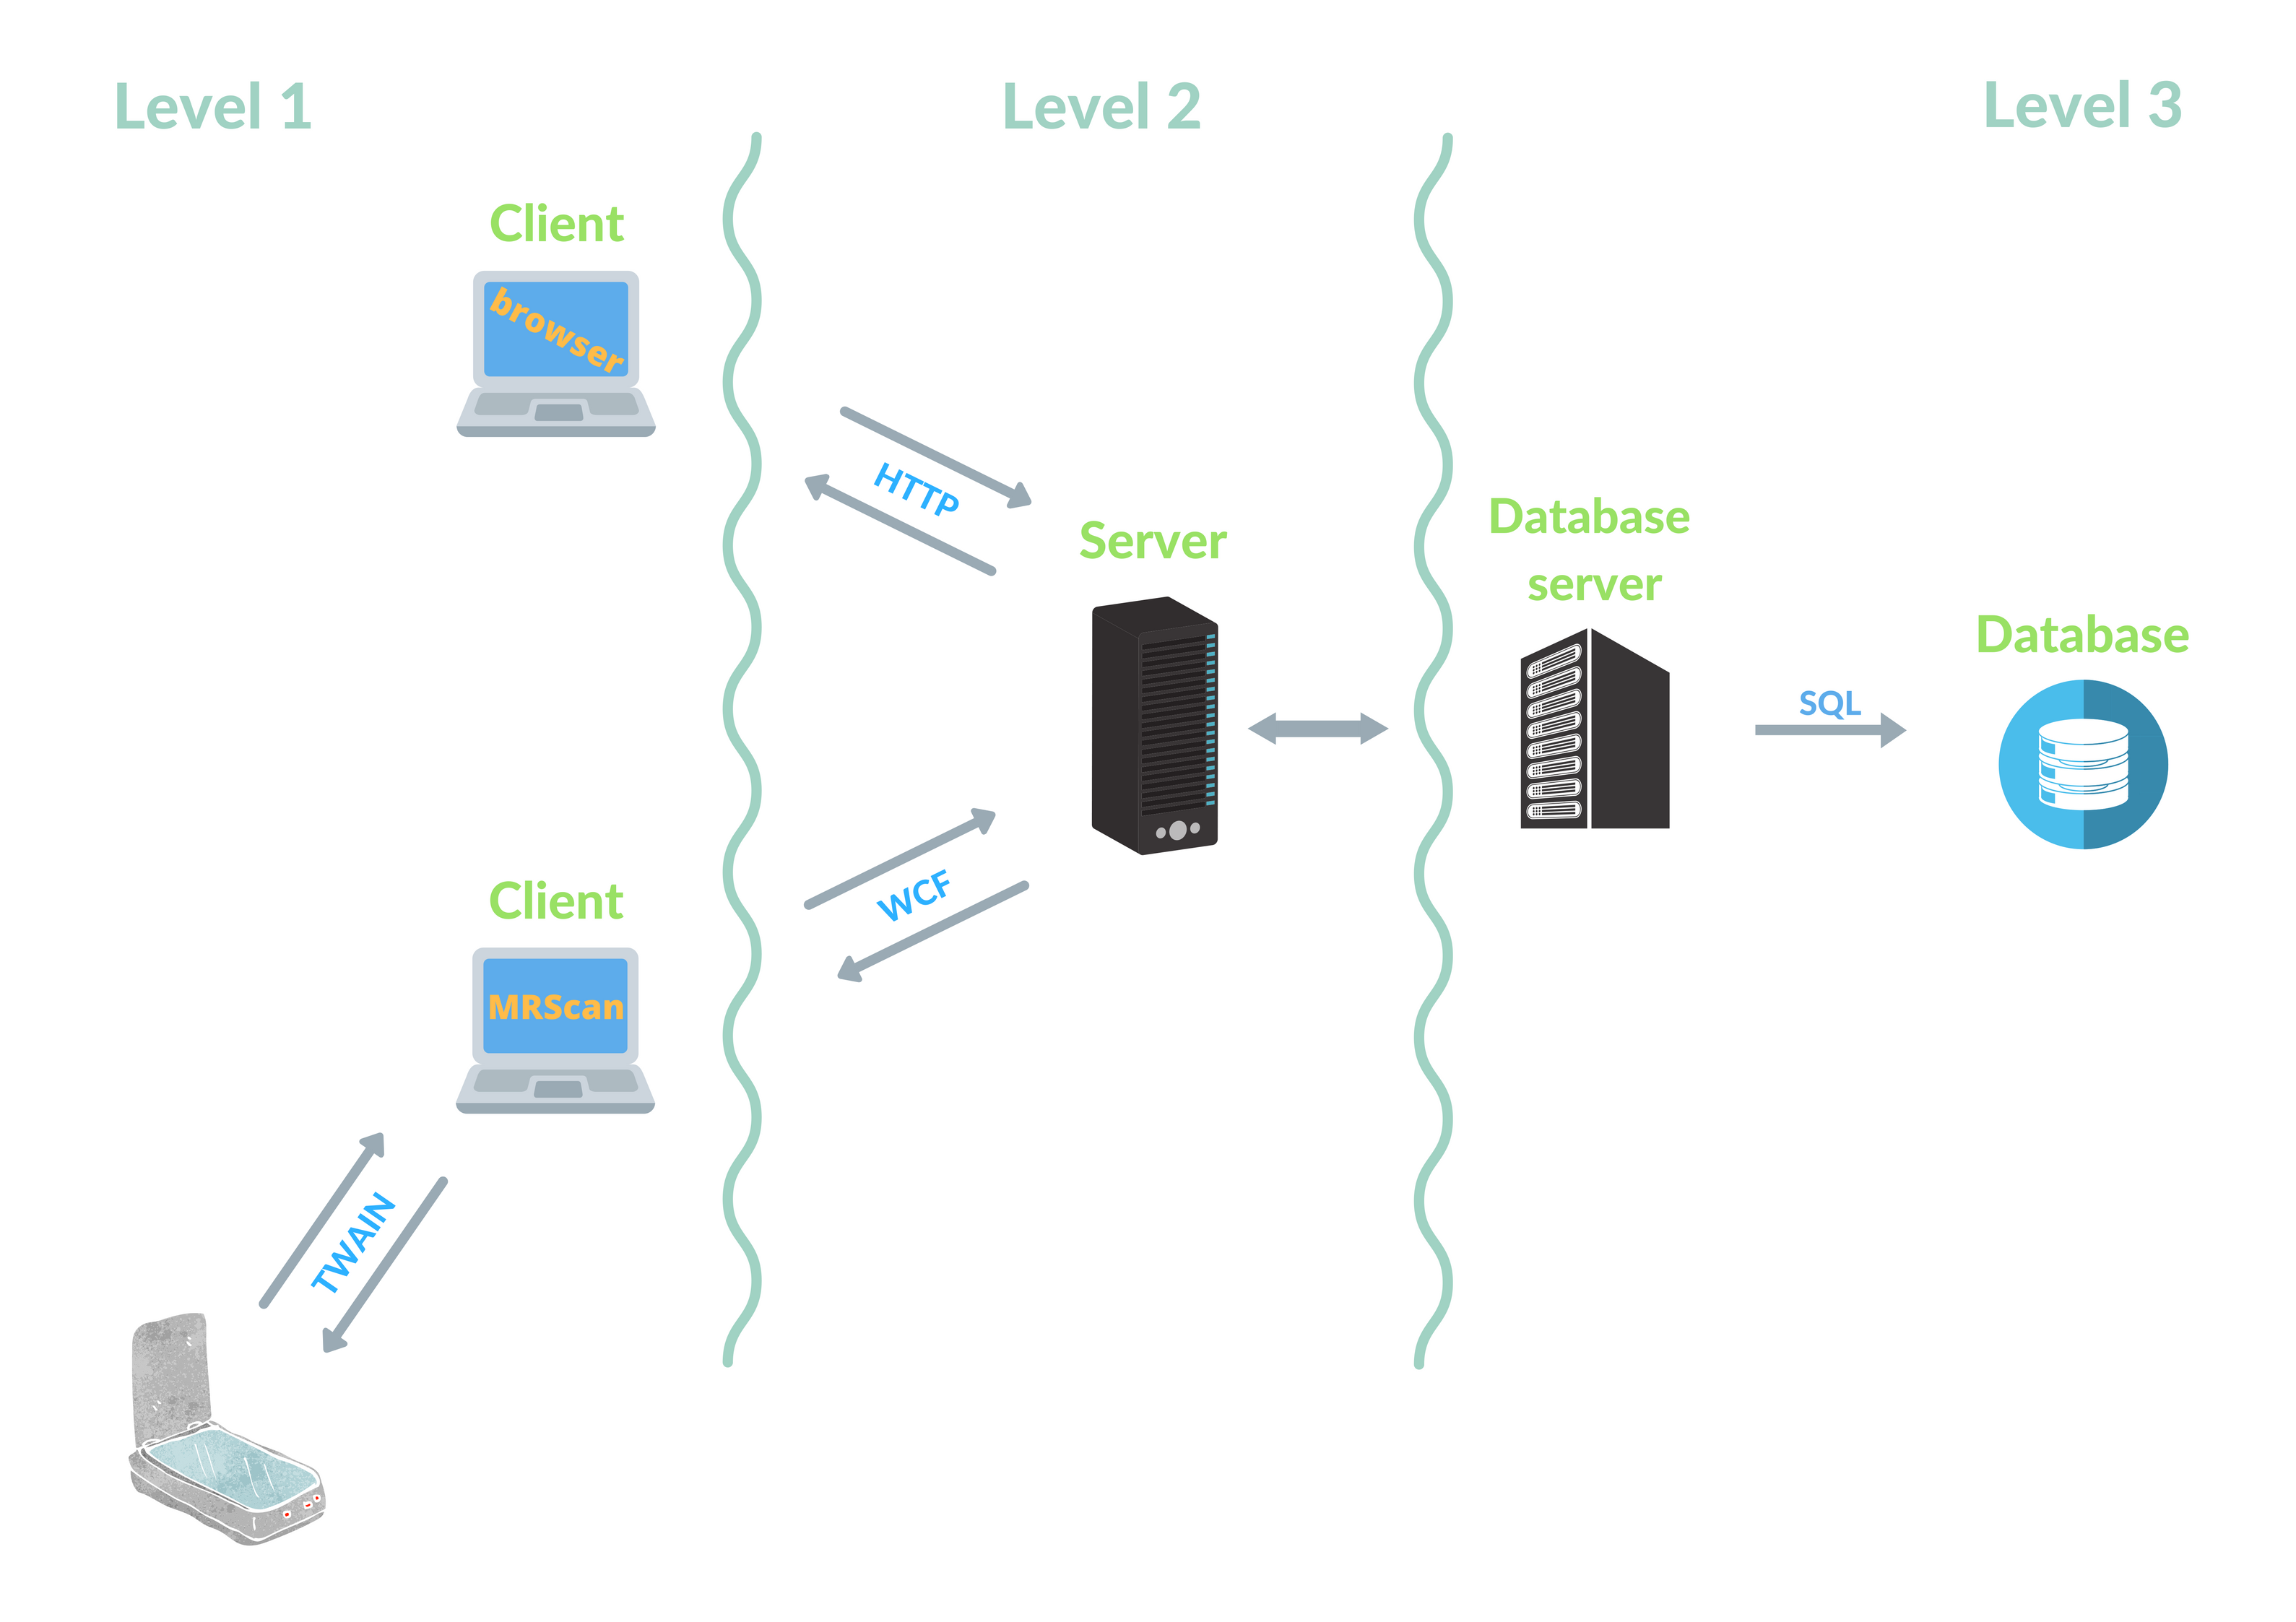
\includegraphics[scale=0.15]{architecture.png}
	\caption{Схема архитектуры проекта}
	\clearpage
\end{figure}